\section{Vector spaces}

    In this and coming sections, all vector spaces can be both finite- or infinite-dimensional. If necessary, the dimension will be specified.

    \newdef{$K$-vector space}{\label{linalgebra:vector_space}
        Let $K$ be a field. A $K$-vector space $V$ is a set equipped with two operations, (vector) addition $V\times V\rightarrow V$ and scalar multiplication $K\times V\rightarrow V$, that satisfy the following axioms (here we put an arrow on top of vectors to make the distinction clear):
        \begin{enumerate}
            \item $V$ forms an Abelian group under vector addition.
            \item Scalar multiplication is associative: $a(b\vec{v}) = (ab)\vec{v}$.
            \item The identity of the field $K$ acts as a neutral element for scalar multiplication: $1_K\vec{v} = \vec{v}$.
            \item Scalar multiplication is distributive with respect to vector addition: $a(\vec{v} + \vec{w}) = a\vec{v} + a\vec{w}$.
        \end{enumerate}
    }

\subsection{Linear independence}

    \newdef{Linear combination}{\label{linalgebra:linear_combination}
        The vector $w$ is a linear combination of elements in the set $\{v_i\}_{i\leq n}$ if it can be written as
        \begin{gather}
            w = \sum_{i=1}^n\lambda_i v_i
        \end{gather}
        for some subset $\{\lambda_i\}_{i\leq n}$ of the field $K$. One can generalize this to general subsets $S\subseteq V$, but the number of nonzero elements $\lambda_i$ should still be finite.\footnote{Generalizations are possible in the context of topological vector spaces (see chapters \ref{chapter:topology} and \ref{chapter:normed_spaces}) where one can define the notion of convergence.}
    }
    \newdef{Linear independence}{\label{linalgebra:linear_independence}
        A finite set $\{v_i\}_{i\leq n}$ is said to be linearly independent if the following relation holds:
        \begin{gather}
            \sum_{i=1}^n\lambda_i v_i = 0 \iff \forall i\leq n:\lambda_i = 0.
        \end{gather}
        A general set $S\subset V$ is linearly independent if every finite subset of it is linearly independent.
    }

    \newdef{Span}{\index{span}
        A set of vectors $S\subseteq V$ is said to span $V$ if every vector $v\in V$ can be written as a linear combination of elements in $S$.
    }

    \newdef{Frame}{\index{frame}
        A $k$-frame is an ordered set of $k$ linearly independent vectors.
    }

\subsection{Bases}

    \newdef{Basis}{
        A set $\mathcal{B}$ is said to be a basis of $V$ if $\mathcal{B}$ is linearly independent and if it spans $V$.
    }
    \begin{property}
        Every set $T$ that spans $V$ contains a basis of $V$.
    \end{property}

    \begin{remark}\index{basis!Schauder}
        In the previous definition we implicitly used the concept of a \textit{Hamel} basis, which is based on two conditions:
        \begin{itemize}
            \item The basis is linearly independent.
            \item Every element in the vector space can be written as a linear combination of a \underline{finite} subset of the basis. (See the first footnote above.)
        \end{itemize}
        Hence, for finite-dimensional spaces we do not have to worry. In infinite-dimensional spaces, however, we have to keep this in mind. An alternative construction, which allows combinations of a countably infinite number of elements, is given by that of a \textit{Schauder basis}.
    \end{remark}

    We now continue by constructing a Hamel basis:
    \begin{construct}[Hamel basis]\index{basis!Hamel}\label{linalgebra:hamel_basis}
        Let $V$ be a vector space over a field $K$ and consider the set of all linearly independent subsets of $V$. Under the relation of inclusion this set becomes a partially ordered set\footnote{See definition \ref{set:poset}.}. Zorn's lemma \ref{set:zorns_lemma} tells us that there exists at least one maximal linearly independent set.

        Now we will show that this maximal subset $S$ is also a spanning set of $V$. Let us choose a vector $v\in V$ that is not already in $S$. From the maximality of $S$ it follows that $S\cup v$ is linearly dependent and hence there exists a finite sequence of numbers $(a^1, \ldots, a^n, b)$ in $K$ and a finite sequence of elements $(e_1, \ldots, e_n)$ in $S$ such that:
        \begin{gather}
            \sum_{i=0}^n a^ie_i + bv = 0
        \end{gather}
        where not all scalars are zero. This then implies that $b\neq0$ because otherwise the set $\{e_i\}_{i\leq n}$ and hence also $S$ would be linearly dependent. It follows that we can write $v$ as\footnote{It is this step that requires $R$ to be a division ring in property \ref{algebra:module_basis} because otherwise we would not generally be able to divide by $b\in R$.}
        \begin{gather}
            v = -\frac{1}{b}\sum_{i=0}^na^ie_i.
        \end{gather}
        Because $v$ was randomly chosen we conclude that $S$ is a spanning set for $V$. It is called a Hamel basis of $V$.
    \end{construct}
    \begin{remark}
        This construction clearly assumes the axiom of choice in set theory, only ZF does not suffice. It can even be shown that the existence of a Hamel basis for every vector space\footnote{This would turn a vector space into a free object in the category of vector spaces.} is equivalent to the axiom of choice (and thus also Zorn's lemma).
    \end{remark}

    \newdef{Dimension}{\index{dimension}\label{linalgebra:dimension}
        Let $V$ be a finite-dimensional $K$-vector space. Let $\mathcal{B}$ be a basis for $V$ that contains $n$ elements. We then define the dimension of $V$ as following:
        \begin{gather}
            \dim(V) := n.
        \end{gather}
    }
    \begin{property}
        Let $V$ be a finite-dimensional $K$-vector space. Every basis of $V$ has the same number of elements.\footnote{This theorem can be generalized to infinite-dimensional spaces by stating that all bases have the same \textit{cardinality}.}
    \end{property}

\subsection{Subspaces}

    \newdef{Subspace}{\label{linalgebra:subspace}
        Let $V$ be a $K$-vector space. A subset $W$ of $V$ is a subspace if $W$ itself is a $K$-vector space under (the restriction of) the operations of $V$. Alternatively we can write this as follows:
        \begin{gather}
            W \leq V\iff \forall w_1, w_2 \in W, \forall \lambda, \mu \in K:\lambda w_1 + \mu w_2 \in W.
        \end{gather}
    }

    \newdef{Grassmannian}{\index{Grassmannian}\label{linalgebra:grassmannian}
        Let $V$ be a $K$-vector space. The set of all subspaces of dimension $k$ is called the Grassmannian $\text{Gr}(k, V)$.
    }
    \begin{property}\label{linalgebra:grassmannian_construction}
        GL$(V)$ acts transitively\footnote{See definition \ref{group:transitive}} on all $k$-dimensional subspaces of $V$. From property \ref{group:transitive_action_property} it follows that the coset space GL$(V)/H_W$ for any stabilizer $H_W$ of some $W\in \text{Gr}(k, V)$ is isomorphic (as a set) to $\text{Gr}(k, V)$.
    \end{property}

    \newdef{Flag}{\index{flag}\index{signature}
        Let $V$ be a finite-dimensional vector space. A sequence of proper subspaces $V_1< \cdots < V_n$ is called a flag of $V$. The sequence $(\dim V_1, \ldots, \dim V_n)$ is called the \textbf{signature} of the flag. If for all $i$, $\dim V_i = i$, the flag is called \textbf{complete}.
    }

    \newdef{Flag variety}{
        The set of all flags of a given signature over a vector space $V$ forms a homogeneous space, called the (generalized) flag variety (of that signature). If the underlying field is the field of real (or complex) numbers then the flag variety is a smooth (or complex) manifold\footnote{See chapter \ref{chapter:manifolds}.}, called the \textbf{flag manifold}.
    }

\subsection{Sum and direct sum}

    \newdef{Sum}{
        \nomenclature[O_zsymbinsum]{$X+Y$}{Sum of the vector spaces $X$ and $Y$.}
        Let $V$ be a $K$-vector space and consider a collection of subspaces $\{W_1,\ldots, W_k\}$. The sum of the subspaces is defined as follows:
        \begin{gather}
            W_1+\cdots+W_k:=\left\{\sum_{i=1}^kw_i : w_i\in W_i\right\}.
        \end{gather}
    }
    \newdef{Direct sum}{\index{direct!sum}\label{linalgebra:direct_sum}
        \nomenclature[O_zsymbinsump]{$X\oplus Y$}{Direct sum of the vector spaces $X$ and $Y$.}
        If every element $v$ of the sum, as defined above, can be written as a unique linear combination then the sum is called a direct sum.
    }
    \newnot{Direct sum}{
        The direct sum of vector spaces is denoted by
        \begin{gather*}
            W_1\oplus\cdots\oplus W_k\equiv\bigoplus_{i=1}^kW_i.
        \end{gather*}
    }

    \begin{formula}
        Let $V$ be a finite-dimensional $K$-vector space and consider two subspaces $W_1, W_2\leq V$. The dimensions of these spaces can be related in the following way:
        \begin{gather}
            \dim(W_1 + W_2) = \dim(W_1) + \dim(W_2) - \dim(W_1\cap W_2).
        \end{gather}
    \end{formula}
    \begin{property}
        Let $V$ be a $K$-vector space and assume that $V$ can be decomposed as $W=W_1\oplus W_2$. If $\mathcal{B}_1$ is a basis of $W_1$ and if $\mathcal{B}_2$ is a basis of $W_2$, then $\mathcal{B}_1\cup\mathcal{B}_2$ is a basis of $W$.
    \end{property}

    \newdef{Complement}{\index{complement}
        Let $V$ be a $K$-vector space and let $W$ be a subspace of $V$. A subspace $W'$ of $V$ is called a complement of $W$ if $V = W\oplus W'$.
    }
    \begin{property}\label{linalgebra:complement}
        Let $V$ be a $K$-vector space and let $U,W$ be two subspaces of $V$. If $V = U+W$ then there exists a subspace $Y\leq U$ such that $V = Y\oplus W$. Furthermore, every subspace $W$ of $V$ has a complement in $V$.
    \end{property}

\subsection{Algebras}

    \newdef{Algebra}{\index{algebra}\label{linalgebra:algebra}
        Let $V$ be a $K$-vector space and let V be equipped with a binary operation $\star: V\times V\rightarrow V$. The tuple $(V,\star)$ is called an algebra over $K$ if it satisfies the following conditions (as in the case of the definition of vector spaces we put an arrow on top of vectors for clarity):
        \begin{enumerate}
            \item Right distributivity: $(\vec{x} + \vec{y})\star\vec{z} = \vec{x}\star\vec{z} + \vec{y}\star\vec{z}$
            \item Left distributivity: $\vec{x}\star(\vec{y} + \vec{z}) = \vec{x}\star\vec{y} + \vec{x}\star\vec{z}$
            \item Compatibility with scalars: $(a\vec{x})\star(b\vec{y}) = ab(\vec{x}\star\vec{y})$
        \end{enumerate}
        These conditions say that the binary operation is bilinear.
    }
    \newdef{Unital algebra}{
        An algebra $V$ is said to be unital if it contains an identity element with respect to the bilinear map $\star$.
    }

    \remark{More generally one can define an algebra over a commutative unital ring $R$. The defining conditions remain the same except that we require $V$ to be an $R$-module instead of a $K$-vector space.}

    \begin{example}[Temperley-Lieb algebra]\index{Temperley-Lieb algebra}\index{Jones!relations}
        \nomenclature[S_TLn]{TL$_n(\delta)$}{Temperley-Lieb algebra with $n-1$ generators and parameter $\delta$.}
        Let $R$ be a commutative unital ring and fix an element $\delta\in R$. The Temperley-Lieb algebra TL$_n(\delta)$ is the unital $R$-algebra with generators $\{U_i\}_{i<n}$ that satisfy the \textbf{Jones relations}:
        \begin{enumerate}
            \item $U_i^2 = \delta U_i$
            \item $U_i U_j = U_j U_i$ if $|i-j|\neq 1$
            \item $U_i U_j U_i = U_i$ if $|i-j| = 1$
        \end{enumerate}
        One can represent the elements of a Temperley-Lieb algebra diagrammatically. All elements of TL$_n(\delta)$ are represented as diagrams with $n$ inputs and $n$ outputs:

        \qquad The unit is given by the diagram where all inputs are connected to the outputs directly across the diagram. The generators $\{U_i\}_{i<n}$ are constructed by connecting the $i^{th}$ input (resp. output) to the $i+1^{th}$ input (resp. output) and all other inputs are connected to the output directly across the diagram.
        Multiplication in TL$_n(\delta)$ is performed diagrammatically by placing two diagrams side by side. Closed loops are replaced by a factor $\delta$.

        \begin{figure}[ht!]
            \centering
            \begin{subfigure}{0.49\textwidth}
                \centering
                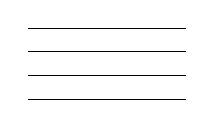
\begin{tikzpicture}
                    \draw (0, 0) -- (2, 0);
                    \draw (0, 0.3) -- (2, 0.3);
                    \draw (0, 0.6) -- (2, 0.6);
                    \draw (0, 0.9) -- (2, 0.9);
                \end{tikzpicture}
                \caption{Unit in TL$_4(\delta)$.}
                \label{fig:unit_temperley_lieb}
            \end{subfigure}
            \begin{subfigure}{0.49\textwidth}
                \centering
                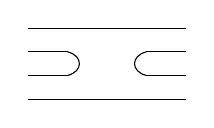
\begin{tikzpicture}
                    \draw (0, 0) -- (2, 0);
                    \draw (0, 0.3) -- (0.5, 0.3);
                    \draw (0, 0.6) -- (0.5, 0.6);
                    \draw (0.5, 0.3) .. controls (0.7, 0.35) and (0.7, 0.55) .. (0.5, 0.6);
                    \draw (1.5, 0.3) -- (2, 0.3);
                    \draw (1.5, 0.6) -- (2, 0.6);
                    \draw (1.5, 0.3) .. controls (1.3, 0.35) and (1.3, 0.55) .. (1.5, 0.6);
                    \draw (0, 0.9) -- (2, 0.9);
                \end{tikzpicture}
                \caption{Generator $U_2$ in TL$_4(\delta)$.}
                \label{fig:generator_temperley_lieb}
            \end{subfigure}
        \end{figure}
    \end{example}

    \begin{example}[Frobenius algebra]\index{Frobenius!algebra}
        An algebra $A$ equipped with a nondegenerate bilinear form $\eta:A\times A\rightarrow A$ satisfying the following condition for all $a,b,c\in A$:
        \begin{gather}
            \eta(ab,c)=\eta(a,bc).
        \end{gather}
    \end{example}

\section[Linear maps]{Linear maps\footnote{Other names are \textbf{linear mapping} and \textbf{linear transformation}.}}
\subsection{Homomorphisms}

    \newdef{Homomorphism space}{\index{morphism!of vector spaces}\label{linalgebra:hom_space}
        \nomenclature[S_Hom]{$\hom(V, W)$}{Space of morphisms from a set $V$ to a set $W$.}
        Let $V,W$ be two $K$-vector spaces. The set of all linear maps between $V$ and $W$ is called the homomorphism space from $V$ to $W$, or shorter the \textbf{hom-space} from $V$ to $W$:
        \begin{gather}
            \hom_K(V, W) := \{f:V\rightarrow W:\text{f is linear}\}.
        \end{gather}
    }
    \begin{formula}\label{linalgebra:hom_dimension}
        If $V,W$ are two finite-dimensional $K$-vector spaces then
        \begin{gather}
            \dim\left(\hom_K(V,W)\right) =\dim(V)\dim(W).
        \end{gather}
    \end{formula}

    \newdef{Endomorphism ring}{
        \nomenclature[S_End]{$\text{End}(V)$}{Ring of endomorphisms on a set $V$.}
        The space $\hom_K(V, V)$ with composition of maps as multiplication forms a ring, the endomorphism ring. It is denoted by $\text{End}_K(V)$ or $\text{End}(V)$ when the underlying field is clear.
    }
    \begin{property}\index{commutator}
        The endomorphism ring $\text{End}(V)$ forms a Lie algebra\footnote{See chapter \ref{chapter:lie} and in particular property \ref{lie:end_as_lie_algebra}.} when equipped with the commutator
        \begin{gather}
            [A, B] = A\circ B - B\circ A.
        \end{gather}
    \end{property}

    \begin{property}[Jordan-Chevalley decomposition]\index{Jordan-Chevalley decomposition}\index{semisimple!operator}\index{nilpotent}\label{linalgebra:jordan_chevalley}
        Every endomorphism $A$ can be decomposed as follows:
        \begin{gather}
            A = A_{ss} + A_n
        \end{gather}
        where
        \begin{itemize}
            \item $A_{ss}$ is \textbf{semisimple}, i.e. for every invariant subspace of $A_{ss}$ there exists an invariant complementary subspace.
            \item $A_n$ is \textbf{nilpotent}, i.e. $\exists k\in\mathbb{N}: A_n^k = 0$.
        \end{itemize}
        Furthermore, this decomposition is unique and the endomorphisms $A_{ss}, A_n$ can be written as polynomials in $A$.
    \end{property}

    \newdef{Minimal polynomial}{\index{minimal!polynomial}
        Let $f\in\text{End}_K(V)$ with $V$ a finite-dimensional $K$-vector space. The monic polynomial $\mu_f(x)$ of lowest order such that $\mu_f(f)=0$ is called the minimal polynomial of $f$.
    }
    \begin{property}\label{linalgebra:minimal_polynomial_divisor}
        Let $f\in\text{End}_K(V)$ with minimal polynomial $\mu_f(x)$ and consider a polynomial $\varphi(x)\in K[x]$. If $\varphi(f) = 0$ then the minimal polynomial $\mu_f(x)$ divides $\varphi(x)$.
    \end{property}

\subsection{Automorphisms}

    \begin{property}
        Let $V$ be finite-dimensional $K$-vector space and let $f:V\rightarrow V$ be an endomorphism. The following statements are equivalent:
        \begin{itemize}
            \item $f$ is injective.
            \item $f$ is surjective.
            \item $f$ is bijective.
        \end{itemize}
    \end{property}

    \newdef{Automorphism}{\index{automorphism}\index{general linear group}\label{linalgebra:automorphism}
        \nomenclature[S_Aut]{$\text{Aut}(V)$}{Set of automorphisms (invertible endomorphisms) on a set $V$.}
        \nomenclature[S_GL]{GL$(V)$}{General linear group: group of all automorphisms on a vector space $V$.}
        An isomorphism from $V$ to $V$ is called an automorphism. The set of all automorphisms  on $V$, which forms in fact a group, is denoted by $\text{Aut}(V)$. In some situations one speaks of the general linear group\footnote{This group is isomorphic to the general linear group of invertible matrices \ref{linalgebra:GL_matrices} (hence the similar name and notation).} GL$_K(V)$ or GL$(V)$ when the underlying field is clear.
    }
    \remark{Sometimes automorphisms are also called \textbf{linear operators}. However, this terminology is also used for a general linear map in operator theory (see chapter \ref{chapter:operator:algebras}) and so we will refrain from using this term.}

    \newdef{Rank}{\index{rank}\label{linalgebra:image_rank}
        The dimension of the image of a linear map.
    }
    \newdef{Kernel}{\index{kernel}
        The kernel of a linear map $f: V \rightarrow W$ is defined as the following subspace of $V$:
        \begin{gather}
            \text{ker}(f) := \{v\in V:f(v) = 0\}.
        \end{gather}
    }
    \newdef{Nullity}{\index{nullity}
        The dimension of the kernel of a linear map.
    }

    \begin{property}
        A linear map $f:V\rightarrow W$ is injective if and only if $\text{ker}(f) = 0$.
    \end{property}
    \begin{property}
        Let $f:V\rightarrow W$ be a linear map and consider a subspace $U\leq V$. The restriction $f|_U$ of $f$ to $U$ has the following two properties:
        \begin{itemize}
            \item $\text{ker}\left(f|_U\right) = \text{ker}(f)\cap U$
            \item $\text{im}\left(f|_U\right) \leq \text{im}(f)$
        \end{itemize}
    \end{property}

    \begin{theorem}[Dimension theorem\footnotemark]\index{rank-nullity theorem}\label{linalgebra:dimension_theorem}
        \footnotetext{Also called the \textbf{rank-nullity theorem}.}
        Let $f: V \rightarrow W$ be a linear map.
        \begin{gather}
            \dim(\text{\upshape im}(f)) + \dim(\text{\upshape ker}(f)) = \dim(\text{\upshape V})
        \end{gather}
    \end{theorem}
    \begin{result}
        Two finite-dimensional vector spaces are isomorphic if and only if they have the same dimension.
    \end{result}

\subsection{Dual maps}

    \newdef{Dual space}{\index{dual!space}
        Let $V$ be a $K$-vector space. The (algebraic) dual $V^*$ of $V$ is defined as the following vector space:
        \begin{gather}
            \label{linalgebra:dual_space}
            V^*:=\text{Hom}_K(V, K)=\{f:V\rightarrow K:f\text{ is a linear map}\}.
        \end{gather}
    }
    \newdef{Linear form}{\index{linear!form}
        The elements of $V^*$ are called linear forms or (linear) functionals.
    }
    \begin{property}\label{linalgebra:dual_space_dimension}
        From theorem \ref{linalgebra:hom_dimension} it follows that $\dim(V^*) = \dim(V)$.
    \end{property}
    \begin{remark}
        If $V$ is infinite-dimensional, theorem \ref{linalgebra:dual_space_dimension} is \underline{never} valid. In the infinite-dimensional case we always have $\text{card}(V^*)>\text{card}(V)$.
    \end{remark}

    \newdef{Dual basis}{
        Let $\mathcal{B} = \{e_1, e_2, \ldots, e_n\}$ be a basis for a finite-dimensional vector space $V$. We can define a basis $\mathcal{B}^* = \{\varepsilon_1, \varepsilon_2, \ldots, \varepsilon_n\}$ for $V^*$, called the dual basis of $\mathcal{B}$, as follows:
        \begin{gather}
            \label{linalgebra:dual_basis}
            \varepsilon_i:\sum_{j=1}^na_ie_i\mapsto a_i.
        \end{gather}
        The relation between a basis and its associated dual basis can also be expressed as
        \begin{gather}
            \label{linalgebra:dual_basis_2}
            \varepsilon^i(e_j) = \delta^i_j.
        \end{gather}
    }

    \newdef{Dual map}{\index{dual!map}\label{linalgebra:transpose}
        Let $f:V\rightarrow W$ be a linear map. The linear map
        \begin{gather}
            f^*:W^*\rightarrow V^*:\varphi\rightarrow\varphi\circ f
        \end{gather}
        is called the dual map or \textbf{transpose} of $f$.
    }

    \newdef{Natural pairing}{\index{natural!pairing}\label{linalgebra:natural_pairing}
        The natural pairing of $V$ and its dual $V^*$ is defined as the following bilinear map:
        \begin{gather}
            \langle v, v^*\rangle := v^*(v).
        \end{gather}
    }

\subsection{Convex functions}

    \newdef{Convex set}{\index{convex}
        A subset of $X$ of a vector space $V$ is said to be convex if $x, y\in X$ implies that $tx = (1-t)y\in X$ for all $t\in[0, 1]$.
    }

    \newdef{Convex function}{
        Let $X$ be a convex subset of $V$. A function $f:X\rightarrow \mathbb{R}$ is said to be convex if for all $x, y\in X$ and $t\in[0, 1]$:
        \begin{gather}
            f(tx + (1-t)y) \leq tf(x) + (1-t)f(y).
        \end{gather}
    }
    \begin{remark}
        For the definition of a \textbf{concave} function we have to turn the inequality around.
    \end{remark}
    \begin{result}
        A linear map $f:X\rightarrow\mathbb{R}$ is both convex and concave.
    \end{result}

    \begin{theorem}[Karamata's inequality]\index{Karamata}
        Let $I\subset\mathbb{R}$ be an interval and let $f:I\rightarrow\mathbb{R}$ be a convex function. If $(x_1, \ldots, x_n)$ is a tuple that majorizes $(y_1, \ldots, y_n)$, i.e. $\forall k\leq n$
        \begin{align}
            \sum_{i=1}^nx_i &= \sum_{i=1}^ny_i\\
            x_{(1)} + \cdots + x_{(k)}&\geq y_{(1)} + \cdots + y_{(k)}
        \end{align}
        where $x_{(i)}$ denotes the ordering\footnote{In decreasing order, i.e. $x_{(1)}\geq\cdots\geq x_{(n)}$.} of the tuple $(x_1, \ldots, x_n)$, then
        \begin{gather}
            \sum_{i=1}^nf(x_i)\geq \sum_{i=1}^nf(y_i).
        \end{gather}
    \end{theorem}
    The following inequality can be proven by induction directly from the definition of convexity:
    \begin{theorem}[Jensen's inequality]\index{Jensen's inequality}
        Let $f$ be a convex function and consider weights $\{a_i\}_{i\leq n}$ such that $\sum_ia_i=1$. Then Jensen's equality states that
        \begin{gather}
            \label{linalgebra:jensen_inequality}
            f\left(\sum_ia_ix_i\right) \leq \sum_ia_if(x_i).
        \end{gather}
    \end{theorem}